% ============================================================
%  IHK Abschlussprüfung 2026
%  Fachinformatiker Anwendungsentwicklung
%  Dokumentation zur betrieblichen Projektarbeit
%
%  Erstellen einer JTL Wawi Cloud App in Form eines BI-Tools
% ============================================================

\documentclass[12pt, a4paper, oneside]{report}

% ── Encoding & Sprache ──────────────────────────────────────
\usepackage[utf8]{inputenc}
\usepackage[T1]{fontenc}
\usepackage[ngerman]{babel}
\usepackage{helvet}
\renewcommand{\familydefault}{\sfdefault}
\usepackage{microtype}

% ── Seitenränder ────────────────────────────────────────────
\usepackage[
  a4paper,
  top=2.5cm,
  bottom=2.5cm,
  left=2.5cm,
  right=2.0cm
]{geometry}

% ── Zeilenabstand ───────────────────────────────────────────
\usepackage{setspace}
\onehalfspacing

% ── Farben ──────────────────────────────────────────────────
\usepackage[dvipsnames, table]{xcolor}
\definecolor{ihkblue}{RGB}{0, 70, 127}
\definecolor{codebg}{RGB}{245, 245, 245}
\definecolor{coderule}{RGB}{180, 180, 180}
\definecolor{linkcolor}{RGB}{0, 90, 160}

% ── Grafiken ────────────────────────────────────────────────
\usepackage{graphicx}
\usepackage{float}
\usepackage{caption}
\captionsetup{skip=4pt}
\usepackage{subcaption}
\graphicspath{{./bilder/}}

% ── Tabellen ────────────────────────────────────────────────
\usepackage{booktabs}
\usepackage{tabularx}
\usepackage{multirow}
\usepackage{longtable}
\usepackage{array}

% ── Code-Listings ───────────────────────────────────────────
\usepackage{listings}
\usepackage{lstautogobble}

\lstdefinestyle{ihkcode}{
  backgroundcolor=\color{codebg},
  basicstyle=\ttfamily\footnotesize,
  breakatwhitespace=false,
  breaklines=true,
  captionpos=b,
  commentstyle=\color{OliveGreen}\itshape,
  frame=single,
  rulecolor=\color{coderule},
  keepspaces=true,
  keywordstyle=\color{MidnightBlue}\bfseries,
  numbers=left,
  numbersep=8pt,
  numberstyle=\tiny\color{gray},
  showspaces=false,
  showstringspaces=false,
  stringstyle=\color{BrickRed},
  tabsize=4,
  autogobble=true,
  xleftmargin=1.5em,
  xrightmargin=0.5em,
  aboveskip=0.5em,
  belowskip=0.3em
}
\lstset{style=ihkcode}

\lstdefinelanguage{JavaScript}{
  keywords={break,case,catch,continue,default,delete,do,else,
    finally,for,function,if,in,new,return,switch,this,throw,
    try,typeof,var,void,while,let,const,class,import,export,async,await},
  sensitive=true,
  comment=[l]{//},
  morecomment=[s]{/*}{*/},
  morestring=[b]',
  morestring=[b]"
}

% ── Kopf- und Fußzeilen (nach Vorlage Feldhaus) ─────────────
\usepackage{fancyhdr}
\usepackage{lastpage}

% Normalseiten-Style
\fancypagestyle{main}{%
  \fancyhf{}
  \fancyhead[L]{%
    \footnotesize\textsc{JTL Wawi Cloud BI-Tool}\\[-2pt]
    \footnotesize Erstellen einer JTL Wawi Cloud App in Form eines BI-Tools
  }
  %\fancyhead[R]{\includegraphics[height=1cm]{logo_ris}}% Logo falls vorhanden
  \fancyfoot[C]{\thepage}
  \renewcommand{\headrulewidth}{0.4pt}
  \renewcommand{\footrulewidth}{0pt}
}

% Kapitelseiten-Style (ohne Logo-Zeile, nur Trennlinie)
\fancypagestyle{chapterstyle}{%
  \fancyhf{}
  \fancyhead[L]{%
    \footnotesize\textsc{JTL Wawi Cloud BI-Tool}\\[-2pt]
    \footnotesize Erstellen einer JTL Wawi Cloud App in Form eines BI-Tools
  }
  \fancyhead[R]{\footnotesize\leftmark}
  \fancyfoot[C]{\thepage}
  \renewcommand{\headrulewidth}{0.4pt}
}

\setlength{\headheight}{28pt}

% ── Verzeichnisse ───────────────────────────────────────────
\usepackage{tocloft}
\renewcommand{\cfttoctitlefont}{\Large\bfseries}
\renewcommand{\cftloftitlefont}{\Large\bfseries}
\renewcommand{\cftlottitlefont}{\Large\bfseries}
\setlength{\cftbeforetoctitleskip}{0pt}
\setlength{\cftbeforeloftitleskip}{0pt}
\setlength{\cftbeforelottitleskip}{0pt}
\setlength{\cftaftertoctitleskip}{6pt}
\setlength{\cftafterloftitleskip}{6pt}
\setlength{\cftafterlottitleskip}{6pt}
\setlength{\cftbeforechapskip}{4pt}
\setlength{\cftbeforesecskip}{1pt}
\setlength{\cftbeforesubsecskip}{0pt}
\setlength{\cftchapindent}{0pt}
\setlength{\cftsecindent}{0pt}
\setlength{\cftsubsecindent}{0pt}
\setlength{\cftsubsubsecindent}{0pt}
\setlength{\cftchapnumwidth}{3.6em}
\setlength{\cftsecnumwidth}{3.6em}
\setlength{\cftsubsecnumwidth}{3.6em}
\setlength{\cftsubsubsecnumwidth}{3.6em}

% ── Abkürzungen ─────────────────────────────────────────────
\usepackage[acronym, toc, nonumberlist, nogroupskip]{glossaries}
\makeglossaries

% ── Literaturverzeichnis ────────────────────────────────────
\usepackage[backend=biber, style=authoryear, sorting=nyt]{biblatex}
\addbibresource{literatur.bib}

% ── Links & PDF-Metadaten ───────────────────────────────────
\usepackage[
  colorlinks=true,
  linkcolor=linkcolor,
  citecolor=linkcolor,
  urlcolor=linkcolor,
  linktoc=page,
  pdftitle={JTL Wawi Cloud BI-Tool -- IHK Abschlussprojekt 2026},
  pdfauthor={Felix Bock},
  pdfsubject={Fachinformatiker Anwendungsentwicklung}
]{hyperref}
\usepackage{bookmark}

% ── Sonstige Pakete ─────────────────────────────────────────
\usepackage{enumitem}
\usepackage{eurosym}
\usepackage{csquotes}
\usepackage{amsmath}
\usepackage{footnote}

% ── Kapitel/Abschnitt-Format (nach Vorlage: seriflos, fett) ─
\usepackage{titlesec}
\titleformat{\chapter}[hang]
  {\normalfont\Large\bfseries}
  {\thechapter}{1em}{}
\titlespacing*{\chapter}{0pt}{20pt}{12pt}

\titleformat{\section}[hang]
  {\normalfont\large\bfseries}
  {\thesection}{1em}{}
\titlespacing*{\section}{0pt}{12pt}{6pt}

\titleformat{\subsection}[hang]
  {\normalfont\normalsize\bfseries}
  {\thesubsection}{1em}{}
\titlespacing*{\subsection}{0pt}{10pt}{4pt}

\titleformat{\subsubsection}[hang]
  {\normalfont\normalsize\bfseries}
  {\thesubsubsection}{1em}{}

% ── Anhang-Nummerierung: A.1, A.2 usw. ─────────────────────
\usepackage{appendix}

% ── Fußnoten ────────────────────────────────────────────────
\usepackage[bottom]{footmisc}

% ============================================================
%  ABKÜRZUNGEN
% ============================================================
\newacronym{api}{API}{Application Programming Interface}
\newacronym{bi}{BI}{Business Intelligence}
\newacronym{ui}{UI}{User Interface}
\newacronym{rest}{REST}{Representational State Transfer}
\newacronym{oauth}{OAuth}{Open Authorization}
\newacronym{jwt}{JWT}{JSON Web Token}
\newacronym{json}{JSON}{JavaScript Object Notation}
\newacronym{spa}{SPA}{Single Page Application}
\newacronym{kpi}{KPI}{Key Performance Indicator}
\newacronym{ihk}{IHK}{Industrie- und Handelskammer}
\newacronym{ris}{RIS}{RIS Web- \& Software-Development GmbH \& Co. KG}
\newacronym{mvp}{MVP}{Minimum Viable Product}
\newacronym{http}{HTTP}{Hypertext Transfer Protocol}
\newacronym{mvc}{MVC}{Model-View-Controller}
\newacronym{orm}{ORM}{Object-Relational Mapping}
\newacronym{ipc}{IPC}{Inter-Process Communication}
\newacronym{cors}{CORS}{Cross-Origin Resource Sharing}
\newacronym{jwk}{JWK}{JSON Web Key}
\newacronym{jwks}{JWKS}{JSON Web Key Set}
\newacronym{hmr}{HMR}{Hot Module Replacement}
\newacronym{css}{CSS}{Cascading Style Sheets}
\newacronym{tsx}{TSX}{TypeScript XML}
\newacronym{jsx}{JSX}{JavaScript XML}
\newacronym{erp}{ERP}{Enterprise Resource Planning}
\newacronym{jtl}{JTL}{JTL-Software GmbH}

% ============================================================
%  PERSÖNLICHE DATEN
% ============================================================
\newcommand{\AutorName}{Felix Bock}
\newcommand{\AutorStrasse}{Ludwig-Erhard-Str. 34}
\newcommand{\AutorOrt}{93077 Bad Abbach}
\newcommand{\Prueflingsnummer}{(166)-95084}
\newcommand{\PruefungsZeitraum}{04.04.2026 - 22.05.2026}
\newcommand{\Ausbildungsbetrieb}{RIS Web- \& Software-Development GmbH \& Co. KG}
\newcommand{\BetriebStrasse}{Siemensstr. 9}
\newcommand{\BetriebOrt}{93049 Regensburg}
\newcommand{\BetreuerName}{[????????]}
\newcommand{\BetreuerTelefon}{[????????]}
\newcommand{\Abgabetermin}{25.05.2026}
\newcommand{\PruefungsJahr}{2026}

% ============================================================
\begin{document}

% ── Römische Seitennummern für Vorseiten ────────────────────
\pagenumbering{Roman}
\pagestyle{empty}

% ============================================================
%  DECKBLATT  (nach Vorlage Feldhaus)
% ============================================================
\begin{titlepage}
  \centering
  \vspace*{3cm}

  % ── Titel ───────────────────────────────────────────────────
  {\LARGE\bfseries Erstellen einer JTL Wawi Cloud App\\[0.4cm]
                   in Form eines BI-Tools}

  \vspace{3cm}

  % ── Autorenblock ────────────────────────────────────────────
  {\normalsize Bericht zur betrieblichen Projektarbeit von}\\[0.5cm]
  {\large\bfseries \AutorName}\\[0.5cm]
  {\normalsize zur Erlangung des Abschlusses}

  \vspace{1.8cm}

  % ── Ausbildungsberuf ────────────────────────────────────────
  {\normalsize als \textbf{Fachinformatiker}}\\[0.25cm]
  {\normalsize\bfseries Fachrichtung}\\[0.25cm]
  {\normalsize\bfseries Anwendungsentwicklung}

  \vfill

  % ── Unternehmensdaten ───────────────────────────────────────
  {\color{ihkblue}\normalsize
    Ausbildungsbetrieb: \Ausbildungsbetrieb\\[0.2cm]
    Projektbetreuer: \BetreuerName\\[0.2cm]
    Prüflingsnummer: \Prueflingsnummer\\[0.2cm]
    Ausführungszeit: \PruefungsZeitraum
  }

  \vspace{1.5cm}
\end{titlepage}

% ============================================================
%  VERZEICHNISSE
% ============================================================
\cleardoublepage
\pagestyle{main}

{\singlespacing\tableofcontents}

{%
  \let\clearpage\relax
  \let\cleardoublepage\relax
  \singlespacing
  \listoffigures
  \addcontentsline{toc}{chapter}{Abbildungsverzeichnis}
  \listoftables
  \addcontentsline{toc}{chapter}{Tabellenverzeichnis}
  \lstlistoflistings
  \addcontentsline{toc}{chapter}{Quelltextverzeichnis}
  \printglossary[type=\acronymtype, title=Abkürzungsverzeichnis]
}

% ── Arabische Seitennummern ab Kapitel 1 ────────────────────
\cleardoublepage
\pagenumbering{arabic}
\setcounter{page}{1}

% ============================================================
%  1  EINLEITUNG
% ============================================================
\chapter{Einleitung}

Die Projektdokumentation schildert den Ablauf des IHK-Abschlussprojektes, welches
im Rahmen der Ausbildung zum Fachinformatiker Anwendungsentwicklung durchgeführt wurde.
Ausbildungsbetrieb ist die \gls{ris} mit Sitz in Regensburg. Das Unternehmen wurde im Jahr 2015
gegründet und beschäftigt derzeit acht Mitarbeiter. Als IT-Dienstleister ist \gls{ris} auf die
Entwicklung individueller Web- und Softwarelösungen spezialisiert und betreut insbesondere
E-Commerce-Unternehmen in Deutschland, Österreich und der Schweiz.
\section{Projektbeschreibung}

Ein zentraler Schwerpunkt der Unternehmenstätigkeit liegt auf der Implementierung und
Erweiterung der Systemlandschaft der JTL-Software. Die JTL-Software-Suite bildet typische
Geschäftsprozesse im Onlinehandel ab. Kernbestandteile sind JTL-Wawi als zentrales
Warenwirtschaftssystem (Artikelverwaltung, Auftragsabwicklung, Lagerverwaltung), Shop- und
Marktplatzanbindungen, über die JTL-Wawi mit externen Verkaufsplattformen wie Amazon oder eBay über standardisierte Datenschnittstellen verbunden wird, sowie cloudbasierte Erweiterungen über die JTL-Cloud.

Aktuell wird die JTL-Wawi schrittweise in eine browserbasierte Umgebung innerhalb der
JTL-Cloud überführt. Diese befindet sich noch in der Beta-Phase und soll perspektivisch
die technologische Grundlage der zukünftigen JTL-Systemlandschaft darstellen. Damit
verbunden ist auch eine neue \gls{api}-Struktur, die externen Anwendungen den Zugriff auf
Geschäftsdaten ermöglichen soll. Viele der von \gls{ris} betreuten Kunden verfügen über
umfangreiche Unternehmensdaten innerhalb der JTL-Wawi, darunter Umsatzdaten, Lagerbestände,
Auftragsvolumen und weitere betriebswirtschaftlich relevante Kennzahlen. Eine flexible,
mobil nutzbare und visuell aufbereitete Auswertung dieser Daten steht derzeit jedoch nicht
zur Verfügung.

In diesem Projekt soll eine \gls{bi}-Applikation als Prototyp entwickelt werden, die diese
Lücke schließt.

\section{Projektziel}

Ziel des Projekts ist die Konzeption und Entwicklung eines Prototypen einer
Business-Intelligence-Applikation zur Visualisierung ausgewählter Geschäftsdaten aus der
JTL-Systemlandschaft. Im Rahmen des Projekts soll die neue \gls{api}-Schnittstelle der
JTL-Cloud analysiert und angebunden werden, um definierte betriebswirtschaftliche Kennzahlen,
beispielsweise Umsätze, Auftragszahlen und Lagerbestände, automatisiert abzurufen.
Die Daten werden strukturiert aufbereitet und in einer benutzerfreundlichen Oberfläche
grafisch dargestellt.

Aufgrund des Beta-Status der JTL-Cloud wird die Anwendung zunächst als Pilotprojekt
umgesetzt. Ziel ist es, die technische Umsetzbarkeit, Stabilität und Integrationsfähigkeit
der Schnittstelle zu bewerten. Sollte sich die Lösung als stabil und praxistauglich
erweisen, besteht die Möglichkeit, diese zu einem marktfähigen Produkt im Portfolio von
\gls{ris} weiterzuentwickeln.

\section{Projektumfeld}

Auftraggeber des Projekts ist die \gls{ris}. Die Ergebnisse richten sich an E-Commerce-Kunden
des Unternehmens, die ihre Geschäftsdaten aus der JTL-Wawi in aufbereiteter Form abrufen
möchten. Darüber hinaus hat \gls{ris} ein strategisches Interesse an einer frühen technischen
Evaluierung der neuen JTL-Cloud-\gls{api}, um die eigene Beratungskompetenz für
cloudbasierte JTL-Erweiterungen auszubauen.

\section{Projektbegründung}


Datengetriebene Unternhemensentscheidungen werden heute in fasst jeder Branche getroffen,
im E-Commerce sind dafür aktuelle Kennzahlen besonders entscheidend.
Ohne eine geeignete Visualisierungsmöglichkeit fehlt Entscheidern
eine kompakte, ortsunabhängige Übersicht über die wirtschaftliche Situation ihres
Unternehmens. Bestehende Auswertungsmöglichkeiten in der JTL-Wawi sind funktional
eingeschränkt oder nicht für eine intuitive, mobile Nutzung ausgelegt.

Für \gls{ris} als JTL-Dienstleister besteht zusätzlich die strategische Notwendigkeit,
die neue Cloud-\gls{api} frühzeitig technisch zu evaluieren und deren Praxistauglichkeit
zu prüfen.

\section{Projektschnittstellen}

Das System kommuniziert über folgende Schnittstellen.
Die Kommunikation mit allen externen Diensten erfolgt verschlüsselt über HTTPS.

\begin{itemize}[leftmargin=1.5em]
  \item \textbf{JTL-Cloud Auth-Server} (\texttt{https://auth.jtl-cloud.com}):
        Stellt über OAuth2, einem offenen Standard zur sicheren Zugriffsautorisierung,
        Zugriffstoken aus. Der verwendete \texttt{client\_credentials}-Flow ist ein
        Server-zu-Server-Verfahren, bei dem die Anwendung sich direkt mit App-ID
        und App-Secret ausweist, ohne dass eine Nutzerinteraktion erforderlich ist.
  \item \textbf{JTL-Cloud API} (\texttt{https://api.jtl-cloud.com}):
        \gls{rest}-\gls{api}, die einen standardisierten Datenaustausch über das
        HTTP-Protokoll ermöglicht, zum Abruf von Geschäftsdaten wie Aufträgen,
        Artikeln und Lagerbeständen
  \item \textbf{Frontend} (React-\gls{spa}): Kommuniziert mit dem eigenen Backend über eine
        interne REST-\gls{api}
\end{itemize}

\section{Projektabgrenzung}

Da der Projektumfang auf 80 Stunden begrenzt ist, sind folgende Punkte ausdrücklich
\textbf{nicht} Bestandteil des Abschlussprojekts:

\begin{itemize}[leftmargin=1.5em]
  \item Entwicklung eines produktionsreifen, marktfähigen Produkts (ausschließlich Prototyp)
  \item Anbindung weiterer Systeme außerhalb der JTL-Cloud-\gls{api}
  \item Mandantenfähigkeit für mehrere gleichzeitige JTL-Kunden
  \item Migration oder Veränderung bestehender JTL-Wawi-Daten
\end{itemize}

% ============================================================
%  2  PROJEKTPLANUNG
% ============================================================
\chapter{Projektplanung}

\section{Projektphasen}

Für die Umsetzung des Projekts standen 80 Stunden zur Verfügung. Diese wurden vor
Projektbeginn auf fünf Hauptphasen verteilt. Eine grobe Übersicht zeigt
Tabelle~\ref{tab:grobe_zeitplanung}. Die detaillierte Zeitplanung findet sich im
Anhang~\ref{anhang:zeitplanung}.

\begin{table}[H]
  \centering
  \caption{Grobe Zeitplanung}
  \label{tab:grobe_zeitplanung}
  \begin{tabularx}{0.6\textwidth}{X r}
    \toprule
    \textbf{Projektphase} & \textbf{Geplante Zeit} \\
    \midrule
    Analysephase          & 10\,h \\
    Entwurfsphase         & 12\,h \\
    Implementierungsphase & 51\,h \\
    Dokumentation         &  5\,h \\
    Abschluss             &  2\,h \\
    \midrule
    \textbf{Gesamt}       & \textbf{80\,h} \\
    \bottomrule
  \end{tabularx}
\end{table}

\section{Ressourcenplanung}

Eine Übersicht der eingesetzten Ressourcen befindet sich im Anhang~\ref{anhang:ressourcen}.
Bei der Auswahl der verwendeten Software wurde auf lizenzkostenfreie Werkzeuge
gesetzt. Open-Source-Software ist zwar quelloffen zugänglich und verursacht keine
Lizenzkosten, ist aber nicht grundsätzlich für alle Nutzungsszenarien kostenlos.
Dadurch sollen anfallende Projektkosten möglichst gering gehalten werden.

\section{Entwicklungsprozess}

Bevor mit der Realisierung des Projekts begonnen werden konnte, musste ein geeigneter
Entwicklungsprozess gewählt werden. Für das Abschlussprojekt wurde ein iterativ-inkrementeller
Ansatz in Anlehnung an agile Vorgehensmodelle gewählt. Die einzelnen Implementierungsphasen
(Backend, Frontend, Qualitätssicherung) werden nacheinander, aber mit regelmäßiger Überprüfung
der Zwischenergebnisse, durchlaufen.

\section{Iterationsplanung}

Auf Basis des gewählten Entwicklungsprozesses wurde vor Beginn der Implementierung
ein Iterationsplan erstellt, der die Umsetzung in folgende Schritte gliedert:

\begin{itemize}[leftmargin=1.5em]
  \item Einrichtung der Entwicklungsumgebung und Projektstruktur
  \item Implementierung der OAuth2-Authentifizierung
  \item Implementierung der JTL-Cloud-\gls{api}-Anbindung (Datenabfragen)
  \item Aufbereitung und Bereitstellung der Daten über die interne \gls{api}
  \item Implementierung der React-Frontend-Komponenten
  \item Implementierung von Filtern und Benutzerinteraktionen
  \item Qualitätssicherung und Code Review
\end{itemize}

Der vollständige Iterationsplan mit Zeitangaben befindet sich im Anhang~\ref{anhang:iterationsplan}.

% ============================================================
%  3  ANALYSEPHASE
% ============================================================
\chapter{Analysephase}

\section{Ist-Analyse}

Wie in Abschnitt~1.1 (Projektbeschreibung) erläutert, fehlt den Kunden von \gls{ris}
derzeit eine mobile, visuell aufbereitete Auswertungsmöglichkeit für ihre JTL-Wawi-Daten.
Die vorhandenen integrierten Analyse-Werkzeuge der JTL-Software sind entweder auf Desktop-Nutzung beschränkt
oder bieten keine flexible Filtermöglichkeit für individuelle Zeiträume und \glspl{kpi}, also messbare Kennzahlen wie Umsatz oder Auftragsanzahl, anhand derer der Geschäftserfolg bewertet wird.

\section{Wirtschaftlichkeitsanalyse}

\subsection{Make-or-Buy-Entscheidung}

Da die Anwendung auf die JTL-Cloud-\gls{api} in ihrer Beta-Phase aufbaut, war eine
Kaufentscheidung strukturell ausgeschlossen: Zum Zeitpunkt der Projektumsetzung existierte
kein Drittanbieterprodukt, das diese Schnittstelle unterstützt. Eine „Buy"-Option stand
damit nicht zur Verfügung. Die Eigenentwicklung bietet zudem den strategischen Vorteil,
dass \gls{ris} frühzeitig Erfahrungswissen mit der neuen JTL-Cloud-Plattform aufbaut,
bevor diese allgemeine Marktreife erlangt, und sich damit als früher Anbieter von
JTL-Cloud-Erweiterungen positioniert.

\subsection{Projektkosten}

Den Berechnungen liegt ein interner Verrechnungssatz von 15\,\EUR{}/h für den
Auszubildenden sowie 25\,\EUR{}/h für Mitarbeiter zugrunde, entsprechend den
betrieblichen Kostensätzen der \gls{ris}.

\begin{table}[H]
  \centering
  \caption{Kostenaufstellung}
  \label{tab:kosten}
  \begin{tabularx}{\textwidth}{X r r r}
    \toprule
    \textbf{Vorgang} & \textbf{Mitarbeiter} & \textbf{Zeit} & \textbf{Gesamt} \\
    \midrule
    Entwicklungskosten  & 1$\times$ Auszubildender & 80\,h & \EUR{1.200,00} \\
    Fachgespräche       & 1$\times$ Mitarbeiter    &  4\,h & \EUR{100,00}   \\
    Code Review         & 1$\times$ Mitarbeiter    &  4\,h & \EUR{100,00}   \\
    Abnahme/Vorstellung & 1$\times$ Mitarbeiter    &  2\,h & \EUR{50,00}    \\
    \midrule
    \textbf{Projektkosten gesamt} & & & \textbf{\EUR{1.450,00}} \\
    \bottomrule
  \end{tabularx}
\end{table}

\subsection{Amortisationsdauer}

Da \gls{ris} die Anwendung als Produkt an JTL-Kunden vermarkten möchte, ergibt sich
die Amortisation nicht aus der Zeitersparnis beim Kunden, sondern aus den zu
erwartenden Lizenzeinnahmen. Als Planungsgrundlage wird folgendes Szenario
zugrunde gelegt: Bei einer monatlichen Lizenzgebühr von 29\,\EUR{} pro Mandant und
fünf zahlenden Kunden beläuft sich der monatliche Deckungsbeitrag auf 145\,\EUR{}.
Bei Projektkosten von 1.450\,\EUR{} ergibt sich eine rechnerische Amortisationsdauer
von zehn Monaten. Dieses Szenario stellt eine konservative Schätzung dar; bei
höherer Kundenzahl oder einem höheren Lizenzpreis verkürzt sich der Zeitraum
entsprechend. Der tatsächliche Lizenzpreis wird nach Abschluss der Beta-Phase auf
Basis von Markt- und Kundenfeedback festgelegt.

\section{Nicht-monetäre Vorteile}

Neben der wirtschaftlichen Rechtfertigung ergeben sich folgende nicht-monetäre Vorteile:

\begin{itemize}[leftmargin=1.5em]
  \item Frühzeitiger Wissensaufbau zur JTL-Cloud-\gls{api} vor deren Marktreife
  \item Stärkung der Wettbewerbsposition von \gls{ris} als JTL-Dienstleister
  \item Verbesserung der Entscheidungsgrundlage für Kunden durch mobile Datenverfügbarkeit
\end{itemize}

\section{Anwendungsfälle}

Die Anwendung richtet sich an Händler, die JTL-Wawi einsetzen. Der primäre
Anwendungsfall ist das Aufrufen des Dashboards, auf dem aggregierte
Geschäftskennzahlen wie Umsatz, Bestellanzahl und Lagerbestand auf einen
Blick dargestellt werden. Daneben ermöglicht die Einrichtungsseite die
einmalige Verbindung der App mit dem JTL-Wawi-Mandanten des Händlers.
Das Pane-Widget zeigt kontextsensitiv die ID des aktuell in der Wawi
ausgewählten Kunden an. Alle drei Anwendungsfälle sind über separate
URL-Pfade (\texttt{/setup}, \texttt{/erp}, \texttt{/pane}) erreichbar
und werden von der JTL-Plattform situationsabhängig aufgerufen.

\section{Lastenheft / Fachkonzept}

Am Ende der Analysephase wurden die Anforderungen des Auftraggebers in einem Lastenheft
festgehalten. Ein Auszug daraus befindet sich im Anhang~\ref{anhang:lastenheft}.

% ============================================================
%  4  ENTWURFSPHASE
% ============================================================
\chapter{Entwurfsphase}

\section{Zielplattform}

Die Applikation wird als JTL Cloud App entwickelt, die sich nahtlos in die
JTL-Cloud-Plattform integriert. Als Architektur wurde eine Monorepo-Struktur gewählt, bei der Frontend und Backend in einem gemeinsamen Quellcode-Repository verwaltet werden und geteilte Konfigurationen sowie koordinierte Builds ermöglicht werden:
ein Express-Backend (TypeScript) übernimmt die Authentifizierung und \gls{api}-Kommunikation,
ein React-Frontend (TypeScript) stellt die Benutzeroberfläche bereit.

Für die Integration in die JTL-Plattform werden folgende JTL-spezifische Pakete eingesetzt:

\begin{itemize}[leftmargin=1.5em]
  \item \textbf{@jtl-software/cloud-apps-core}: AppBridge, die plattformeigene
        Kommunikationsschicht zwischen der eingebetteten App und dem JTL-Host-System,
        für \gls{ipc}-Kommunikation mit der JTL-Wawi
  \item \textbf{@jtl-software/platform-ui-react}: Bibliothek vorgefertigter
        UI-Komponenten, die wiederverwendbare visuelle Bausteine wie Schaltflächen
        oder Tabellen im JTL-Design-System bereitstellt
\end{itemize}

Für die Verifikation der von der JTL-Plattform ausgestellten \glspl{jwt} wird
die Open-Source-Bibliothek \textbf{jose} eingesetzt. Da die JTL-Plattform ihre
Token mit dem EdDSA-Algorithmus signiert, einem asymmetrischen Signaturverfahren
auf Basis elliptischer Kurven, war eine Bibliothek mit vollständiger EdDSA-Unterstützung
erforderlich. \textbf{jose} ist kein JTL-eigenes Paket, sondern eine
plattformunabhängige \gls{jwt}-Bibliothek, die für diesen Anwendungsfall gewählt wurde.

Das Frontend-Framework war durch die JTL-Plattform technisch vorgegeben: Das offizielle
JTL-Paket \texttt{@jtl-software/platform-ui-react} stellt ausschließlich React-spezifische
UI-Komponenten bereit, und die AppBridge-Integration in \texttt{@jtl-software/cloud-apps-core}
setzt React-Hooks voraus. Der Einsatz eines anderen Frameworks hätte die Kompatibilität
mit diesen Plattformpaketen ausgeschlossen, weshalb eine Alternativbewertung entfällt.
Darüber hinaus fügt sich \textbf{React} inhaltlich gut in das Projekt ein: Die verwendete
Diagrammbibliothek \textbf{Recharts} ist eine React-native Bibliothek und ist unmittelbar auf
Dashboard-Anwendungsfälle ausgelegt. \textbf{React} bietet erstklassige TypeScript-Unterstützung,
was angesichts des durchgehenden TypeScript-Einsatzes im gesamten Monorepo die
Konsistenz erhöht. Schließlich begünstigte die weite Verbreitung von \textbf{React} den engen
Zeitrahmen von 80\,h, da auf eine umfangreiche Dokumentation und erprobte Lösungsmuster
zurückgegriffen werden konnte.

Für das Backend-Framework wurde eine Nutzwertanalyse\footnote{Vgl.
Anhang~\ref{anhang:nutzwert}.} zwischen den JavaScript-Frameworks
\textbf{Express}, \textbf{NestJS} und \textbf{Fastify} durchgeführt, da alle drei
im gleichen Ökosystem (\textbf{Node.js} / \textbf{TypeScript}) betrieben werden und somit eine
vergleichbare Grundlage bilden. Die Gewichtung (Gew.) spiegelt die Bedeutung
des jeweiligen Kriteriums für dieses Projekt wider; der Höchstwert 5 bedeutet
unverzichtbar, 1 bedeutet vernachlässigbar. Die Bewertung (Bew.) gibt an, wie
gut ein Framework das Kriterium erfüllt: 5 = sehr gut, 1 = unzureichend. Der
Nutzwert errechnet sich als Quotient aus der gewichteten Gesamtpunktzahl und der
Summe aller Gewichtungen.

\begin{table}[H]
  \centering
  \caption{Nutzwertanalyse zur Auswahl des Backend-Frameworks}
  \label{tab:nutzwert}
  \begin{tabularx}{\textwidth}{l r r r r r r r}
    \toprule
    \textbf{Kriterium} & \textbf{Gew.} &
    \multicolumn{2}{c}{\textbf{Express}} &
    \multicolumn{2}{c}{\textbf{NestJS}} &
    \multicolumn{2}{c}{\textbf{Fastify}} \\
    & & Bew. & Gew. & Bew. & Gew. & Bew. & Gew. \\
    \midrule
    Bibliotheks-Kompatibilität & 5 & 5 & 25 & 4 & 20 & 5 & 25 \\
    Einarbeitungsaufwand       & 5 & 5 & 25 & 2 & 10 & 4 & 20 \\
    TypeScript-Unterstützung   & 4 & 4 & 16 & 5 & 20 & 5 & 20 \\
    Kenntnisstand              & 4 & 5 & 20 & 2 &  8 & 2 &  8 \\
    Prototyp-Eignung           & 4 & 5 & 20 & 2 &  8 & 4 & 16 \\
    \midrule
    \textbf{Gesamt:} & \textbf{22} & & \textbf{106} & & \textbf{66} & & \textbf{89} \\
    \textbf{Nutzwert:} & & & \textbf{4,82} & & \textbf{3,00} & & \textbf{4,05} \\
    \bottomrule
  \end{tabularx}
\end{table}

\textbf{Express} erzielt mit einem Nutzwert von 4{,}82 das beste Ergebnis und wird daher
für das Backend eingesetzt. Die fünf Kriterien wurden wie folgt gewichtet und
bewertet:

\textbf{Bibliotheks-Kompatibilität (Gew. 5):} Die im Backend verwendeten Pakete
\texttt{jose} und \texttt{graphql-request} sind Standard-npm-Pakete, die mit
jedem Node.js-Framework funktionieren. \textbf{Express} erhält die volle Punktzahl, da
es der am weitesten verbreitete Standard ist, für den alle Bibliotheken primär
getestet sind; \textbf{NestJS} erhält einen Punkt Abzug, weil die zusätzliche
Abstraktionsschicht gelegentlich Anpassungen erfordert.

\textbf{Einarbeitungsaufwand (Gew. 5):} Innerhalb des 80-Stunden-Zeitbudgets
war minimaler Overhead entscheidend. \textbf{Express} erfordert kein
Framework-spezifisches Architekturmuster und erlaubt den sofortigen Einstieg.
\textbf{NestJS} verlangt Kenntnisse in Decorators, Dependency Injection und
Modulstrukturen, was für einen Prototyp unverhältnismäßig aufwändig ist und
daher mit 2 bewertet wird.

\textbf{TypeScript-Unterstützung (Gew. 4):} \textbf{TypeScript} ist im gesamten
Monorepo durchgehend eingesetzt. \textbf{NestJS} und \textbf{Fastify} sind TypeScript-first
entwickelt (Bewertung 5), während \textbf{Express} auf Community-Typings
(\texttt{@types/express}) angewiesen ist (Bewertung 4).

\textbf{Kenntnisstand (Gew. 4):} \textbf{Express} war aus früheren Projekten bereits
bekannt, was die Implementierungszeit direkt verkürzt (Bewertung 5).
\textbf{NestJS} und \textbf{Fastify} waren neu und hätten zusätzliche Einarbeitungszeit
erfordert (Bewertung 2).

\textbf{Prototyp-Eignung (Gew. 4):} \textbf{Express} erlaubt es, Endpunkte ohne
Boilerplate direkt zu definieren. \textbf{NestJS} ist als Enterprise-Framework für einen
Prototyp überdimensioniert und erhält daher die niedrigste Bewertung (2).
\textbf{Fastify} liegt mit seinem schlanken Plugin-System dazwischen (Bewertung 4).

\section{Architekturdesign}

Das Projekt wird auf Basis einer \textbf{Client-Server-Architektur} umgesetzt.
Das Backend übernimmt Datenbeschaffung, Authentifizierung und die Kommunikation
mit der JTL-Cloud-\gls{api}; das Frontend ist ausschließlich für die Darstellung
und Benutzerinteraktion zuständig. Die Trennung von Datenzugriff und Darstellung
orientiert sich an bewährten Architekturprinzipien und erleichtert die
unabhängige Weiterentwicklung beider Schichten.

Eine JTL-Cloud App ist eine vom Entwickler eigenständig gehostete
Webanwendung, die über den JTL App Shell als sandboxierter \texttt{iframe}
in die browserbasierte JTL-Cloud-Oberfläche eingebettet wird; ein
\texttt{iframe} stellt dabei einen eingebetteten Browser-Rahmen dar, der
eine separate Webanwendung innerhalb der JTL-Cloud isoliert ausführt.
Der App Shell übernimmt dabei Authentifizierungstoken-Verwaltung und Kommunikation
mit dem Host-System, also der JTL-Cloud-Oberfläche, die den Rahmen
für den \texttt{iframe} bereitstellt;
die eigentliche Anwendungslogik verbleibt vollständig auf der Seite des
Entwicklers. Jeder Händler, der die App installiert, stellt einen eigenen
\textbf{Tenant} dar. Die Datenisolation zwischen Mandanten ist durch das
Plattformmodell sichergestellt.

Die Kommunikation zwischen App Shell und dem eingebetteten Frontend erfolgt
über die \gls{jtl} AppBridge (\texttt{@jtl-software/cloud-apps-core}), welche
das plattformeigene \gls{ipc}-Protokoll kapselt. Über die AppBridge werden
Session-Tokens übermittelt sowie Methoden und Events der JTL-Wawi abgerufen.

\begin{figure}[H]
  \centering
  \fcolorbox{ihkblue}{codebg}{\parbox{0.82\textwidth}{\centering\vspace{0.5cm}
    %
    \textbf{JTL-Cloud-Plattform}\\[0.05cm]
    {\small\texttt{auth.jtl-cloud.com} ~$\cdot$~ \texttt{api.jtl-cloud.com/erp/v2/graphql}}\\[0.3cm]
    %
    $\updownarrow$\\[-0.1cm]
    {\small OAuth2 (\texttt{client\_credentials}) + \gls{jwks} ~$\cdot$~ GraphQL-Abfragen}\\[0.3cm]
    %
    \textbf{Express-Backend (TypeScript)}\\[0.05cm]
    {\small Session-Token-Verifikation ~$\cdot$~ GraphQL-Proxy ~$\cdot$~ Tenant-Mapping}\\[0.3cm]
    %
    $\updownarrow$\\[-0.1cm]
    {\small interne \gls{api} (\texttt{/connect-tenant}, \texttt{/graphql})}\\[0.3cm]
    %
    \textbf{React-Frontend (TypeScript)}\\[0.05cm]
    {\small Setup-Seite ~$\cdot$~ Dashboard ~$\cdot$~ Pane-Widget}\\[0.3cm]
    %
    $\updownarrow$\\[-0.1cm]
    {\small AppBridge (\gls{ipc})}\\[0.3cm]
    %
    \textbf{JTL-Wawi / JTL App Shell}\\[0.05cm]
    {\small Session-Token ~$\cdot$~ Events ~$\cdot$~ Methoden}
    \vspace{0.5cm}
  }}
  \caption{Systemarchitektur, Übersicht}
  \label{fig:architektur}
\end{figure}

\begin{figure}[H]
  \centering
  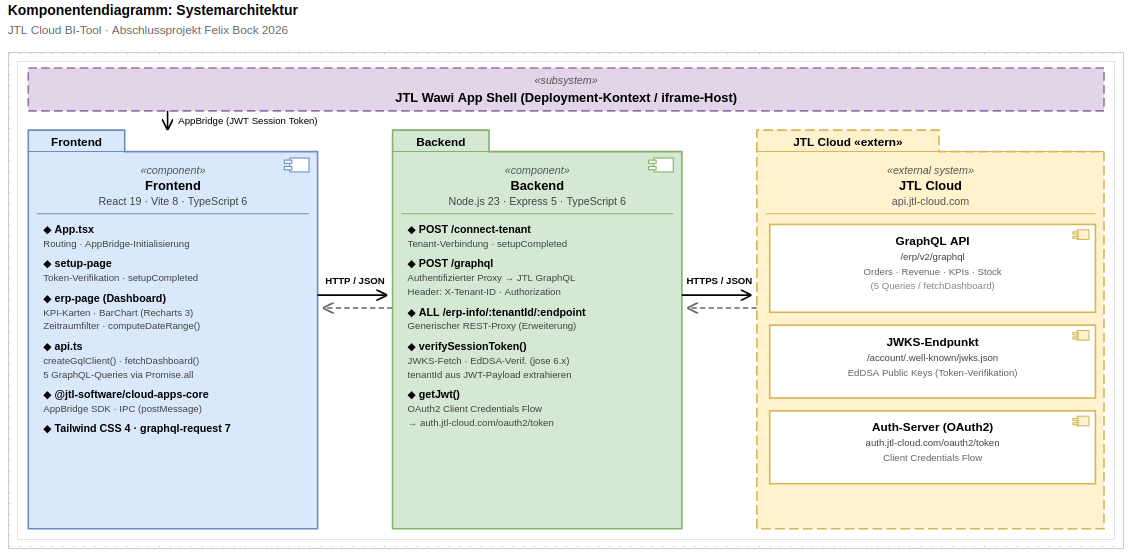
\includegraphics[width=0.95\textwidth]{image3}
  \caption{Komponentendiagramm der Systemarchitektur}
  \label{fig:komponenten}
\end{figure}

\section{Entwurf der Benutzeroberfläche}

Um die Anwendung möglichst benutzerfreundlich zu gestalten, wurde zunächst ein Prototyp
der Oberfläche als Mockup angefertigt. Dabei wurde auf eine klare, übersichtliche
Darstellung der \glspl{kpi} geachtet. Die Dashboard-Hauptansicht zeigt Karten für
Umsatz und Auftragszahlen sowie ein Balkendiagramm für den Umsatzverlauf der
letzten sieben Tage und eine Auflistung der jüngsten Bestellungen. Mockups befinden sich im Anhang~\ref{anhang:mockups}.

\section{Datenmodell und API-Kommunikation}

\subsection{Selbst implementierte Backend-Endpunkte}

Im Rahmen des Projekts wurden im Express-Backend folgende eigene \gls{api}-Endpunkte
implementiert, über die das Frontend alle Anfragen abwickelt. Sie bilden eine
Zwischenschicht zwischen Frontend und JTL-Cloud-\gls{api} und übernehmen
Authentifizierung, Token-Verifikation und Weiterleitung.

Die JTL-Cloud-\gls{api} stellt neben klassischen REST-Endpunkten eine
GraphQL-Schnittstelle bereit. GraphQL ist eine Abfragesprache für \glspl{api},
bei der der Client exakt vorgibt, welche Felder zurückgegeben werden sollen,
anstatt fest definierte Antwortstrukturen zu empfangen. Für das Dashboard
wurde diese Schnittstelle bewusst gewählt: Die fünf Anzeigebereiche des
Dashboards benötigen jeweils unterschiedliche Daten aus unterschiedlichen
API-Ressourcen. Mit GraphQL lassen sich diese fünf Abfragen über einen
einzigen Backend-Endpunkt (\texttt{/graphql}) abwickeln, ohne dass für
jeden Anzeigebereich ein eigener REST-Endpunkt implementiert werden müsste.
Zusätzlich verhindert das feldgenaue Abfragen das Übertragen nicht benötigter
Daten (Over-Fetching).

\begin{table}[H]
  \centering
  \caption{Selbst implementierte Backend-\gls{api}-Endpunkte}
  \label{tab:api_endpunkte}
  \begin{tabularx}{\textwidth}{l l X}
    \toprule
    \textbf{Methode} & \textbf{Pfad} & \textbf{Beschreibung} \\
    \midrule
    POST & \texttt{/connect-tenant} & Verifikation des Session-Tokens und Tenant-Mapping \\
    POST & \texttt{/graphql} & Authentifizierter GraphQL-Proxy zur JTL-Cloud-\gls{api} \\
    ANY  & \texttt{/erp-info/:tenantId/:endpoint} & Generischer REST-Proxy zur JTL-Cloud-\gls{api} (alle HTTP-Methoden) \\
    \bottomrule
  \end{tabularx}
\end{table}

Das Dashboard ruft alle Daten über den \texttt{/graphql}-Proxy in einer einzigen
Funktion (\texttt{fetchDashboard}) ab. Die fünf dabei eingesetzten GraphQL-Operationen
sowie ihre Rückgabetypen sind in Tabelle~\ref{tab:datenmodell} aufgeführt.

\begin{table}[H]
  \centering
  \caption{GraphQL-Operationen und Rückgabetypen}
  \label{tab:datenmodell}
  \begin{tabularx}{\textwidth}{l l X}
    \toprule
    \textbf{Operation} & \textbf{Variablen} & \textbf{Rückgabefelder} \\
    \midrule
    \texttt{DashboardKPIs}      & \texttt{\$from}, \texttt{\$to}
      & \texttt{totalRevenue}, \texttt{totalOrders},
        \texttt{totalCustomers}, \texttt{avgOrderValue} \\
    \texttt{RevenueGrouped}     & \texttt{\$from}, \texttt{\$to}, \texttt{\$groupBy}
      & \texttt{label}, \texttt{revenue}, \texttt{orders} \\
    \texttt{TopItemsByRevenue}  & ---
      & \texttt{sku}, \texttt{name}, \texttt{stockInOrders},
        \texttt{salesPriceGross}, \texttt{totalRevenue} \\
    \texttt{QuerySalesOrders}   & ---
      & \texttt{salesOrderNumber}, \texttt{salesOrderDate},
        \texttt{totalGrossAmount}, \texttt{companyName}, \texttt{status} \\
    \texttt{LowStockItems}      & ---
      & \texttt{sku}, \texttt{name}, \texttt{quantityTotal},
        \texttt{quantityAvailable}, \texttt{quantityLockedForShipment} \\
    \bottomrule
  \end{tabularx}
\end{table}

Die Feldnamen entsprechen direkt den tatsächlichen Feldnamen der JTL-Cloud-GraphQL-\gls{api};
sie werden ohne eigene Modellierung als TypeScript-Interfaces in \texttt{api.ts}
abgebildet. Variablen für Zeitraumangaben (\texttt{\$from}, \texttt{\$to},
\texttt{\$groupBy}) werden von der Hilfsfunktion \texttt{computeDateRange()} berechnet
und als \gls{api}-Variablen übergeben.

\subsection{JTL AppBridge-Kommunikation}

Die Kommunikation zwischen der App und der JTL-Wawi erfolgt über die
JTL AppBridge, einer \gls{ipc}-Schnittstelle. Tabelle~\ref{tab:appbridge_methods}
zeigt die verfügbaren Methoden und Events.

\begin{table}[H]
  \centering
  \caption{AppBridge-Methoden und Events}
  \label{tab:appbridge_methods}
  \begin{tabularx}{\textwidth}{l l X}
    \toprule
    \textbf{Typ} & \textbf{Name} & \textbf{Beschreibung} \\
    \midrule
    Method & \texttt{getSessionToken} & Ruft das aktuelle Session-Token ab \\
    Method & \texttt{setupCompleted} & Signalisiert erfolgreiche App-Einrichtung \\
    Method & \texttt{getCurrentCustomerId} & Gibt die aktuelle Kunden-ID zurück \\
    Event  & \texttt{CustomerChanged} & Wird bei Kundenauswahl ausgelöst \\
    \bottomrule
  \end{tabularx}
\end{table}

\subsection{OAuth2-Authentifizierungskonzept}

Die JTL-Cloud-\gls{api} erfordert eine OAuth2-Authentifizierung nach dem
\texttt{client\_credentials}-Flow.\footnote{Vgl. JTL-Software GmbH [2026].}
Das Backend sendet dabei \texttt{CLIENT\_ID} und \texttt{CLIENT\_SECRET} als
Base64-kodierte Basic-Auth-Kombination an \url{https://auth.jtl-cloud.com/oauth2/token}
und erhält im Gegenzug ein kurzlebiges Access-Token zurück. Dieses Token wird bei
jedem Aufruf der JTL-Cloud-\gls{api} als \texttt{Authorization: Bearer}-Header
mitgeschickt. Client-Daten werden ausschließlich als Umgebungsvariablen im Backend
gehalten und sind nie im Frontend sichtbar. Der vollständige Quellcode der Funktion
\texttt{getJwt()} befindet sich in Anhang~\ref{anhang:quellcode}.
Abbildung~\ref{fig:sequenz} zeigt den vollständigen Ablauf vom Session-Token-Empfang
bis zur verifizierten Tenant-Zuordnung.

\begin{figure}[H]
  \centering
  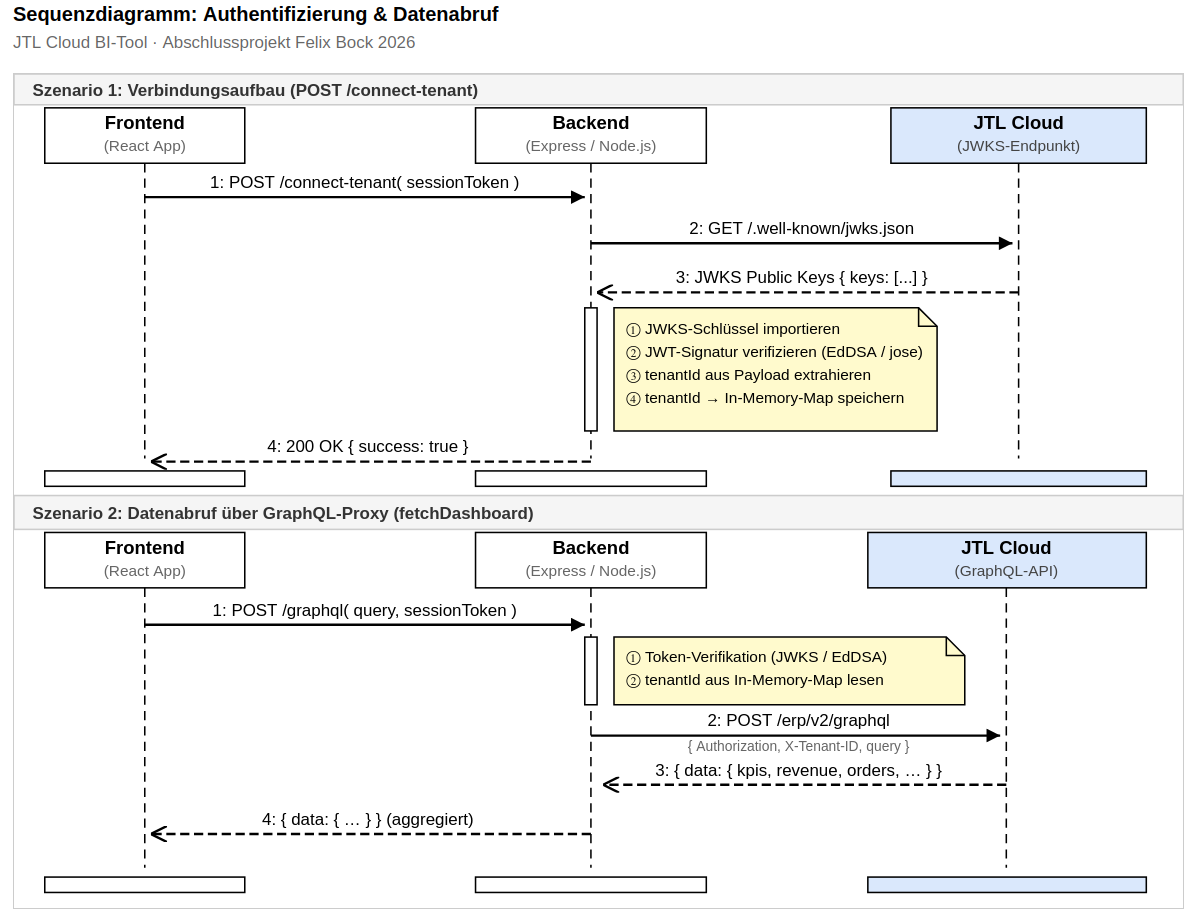
\includegraphics[width=0.95\textwidth]{image2}
  \caption{Sequenzdiagramm: Authentifizierungs- und Token-Verifikationsablauf}
  \label{fig:sequenz}
\end{figure}

\section{Pflichtenheft}

Am Ende der Entwurfsphase wurde ein Pflichtenheft erstellt, das beschreibt, wie und
womit die Anforderungen des Lastenhefts umgesetzt werden. Ein Auszug befindet sich
im Anhang~\ref{anhang:pflichtenheft}.

% ============================================================
%  5  IMPLEMENTIERUNGSPHASE
% ============================================================
\chapter{Implementierungsphase}

\section{Implementierung der Projektstruktur}

Zu Beginn der Implementierungsphase wurde die Projektstruktur angelegt.

\begin{lstlisting}[language=bash, caption={Projektstruktur}, label=lst:struktur]
jtl-cloud-bi-app/
|-- packages/
|   |-- backend/                   # Express-Backend
|   |   |-- src/
|   |   |   |-- index.ts           # Server-Einstiegspunkt
|   |   |   |-- constants.ts       # Umgebungskonstanten
|   |   |-- package.json
|   |   |-- tsconfig.json
|   |-- frontend/                  # React-Frontend
|       |-- src/
|       |   |-- pages/
|       |   |   |-- setup-page/    # App-Setup-Seite
|       |   |   |-- erp-page/      # ERP-Integrationsseite
|       |   |   |-- pane-page/     # Seitenleisten-Widget
|       |   |-- common/            # Gemeinsame Utilities
|       |   |-- App.tsx            # Haupt-App-Komponente
|       |   |-- main.tsx           # React-Einstiegspunkt
|       |-- package.json
|-- turbo.json                     # Monorepo-Orchestrierung
|-- package.json
\end{lstlisting}

\section{Implementierung der Geschäftslogik}

Da die Implementierung der OAuth2-Authentifizierung und der \gls{api}-Anbindung den
Kernbestandteil des Projekts darstellt, soll diese im Folgenden genauer erläutert werden.

\subsection{Session-Token-Verifikation}

Wenn der Händler die App zum ersten Mal öffnet, liefert die JTL AppBridge über
\texttt{getSessionToken()} ein vom JTL-Auth-Server signiertes \gls{jwt}.
Das Backend verifiziert dieses Token in drei Schritten: Zunächst ruft es
die öffentlichen Schlüssel vom \gls{jwks}-Endpunkt
(\url{https://api.jtl-cloud.com/account/.well-known/jwks.json}) ab.
Anschließend wird der passende Schlüssel über die Bibliothek \texttt{jose}
in ein \texttt{CryptoKey}-Objekt importiert. Schließlich prüft \texttt{jwtVerify()}
Signatur, Aussteller und Ablaufzeit des Tokens und extrahiert aus dem Payload
die \texttt{tenantId}, die zur Identifikation des Mandanten genutzt wird.
Ein ungültiges oder abgelaufenes Token führt zu einem sofortigen Abbruch mit
HTTP-Statuscode 401. Die vollständige Implementierung zeigt
Listing~\ref{lst:tokenmanager} im Anhang.

\subsection{ERP-API-Proxy}

Das Backend stellt unter \texttt{/erp-info/:tenantId/:endpoint} einen generischen
REST-Proxy bereit. Dieser nimmt beliebige HTTP-Methoden entgegen, ergänzt den
OAuth2-Bearer-Token im Header sowie die \texttt{X-Tenant-ID} zur Mandantenisolation
und leitet die Anfrage an \url{https://api.jtl-cloud.com/erp/} (+ Endpunkt-Pfad) weiter.
Der Endpunkt ist bewusst generisch gehalten, damit künftige Erweiterungen weitere
JTL-Cloud-REST-Ressourcen anbinden können, ohne Änderungen am Backend vorzunehmen.
Der vollständige Quellcode befindet sich in Listing~\ref{lst:apiservice} im Anhang.

\subsection{GraphQL-Datenabruf}
\label{sec:graphql}

Das zentrale Dashboard bezieht alle Anzeigedaten ausschließlich über den
\texttt{/graphql}-Endpunkt des Backends, der als authentifizierter Proxy zur
JTL-Cloud-GraphQL-Schnittstelle
(\url{https://api.jtl-cloud.com/erp/v2/graphql}) fungiert.
Der vollständige Datenweg vom Öffnen des Dashboards bis zur Anzeige läuft
wie folgt ab: Die React-Komponente ruft beim Laden über die AppBridge das
aktuelle Session-Token ab und übergibt es an \texttt{fetchDashboard()}.
Diese Funktion erstellt mit \texttt{createGqlClient()} einen
\texttt{graphql-request}-Client, der das Token im \texttt{X-Session-Token}-Header
mitführt. Das Backend empfängt die Anfrage, prüft das Token per
\gls{jwks}-Verifikation, holt sich über den OAuth2-\texttt{client\_credentials}-Flow
ein Access-Token und leitet die GraphQL-Abfragen mit diesem Bearer-Token an
die JTL-Cloud-\gls{api} weiter. Die Antwort wird an das Frontend
zurückgegeben und dort in den Komponentenzustand übertragen.

Da die fünf Queries voneinander unabhängig sind, werden sie parallel über
\texttt{Promise.all} ausgeführt. Bei sequenzieller Ausführung würde die
Wartezeit aller fünf Anfragen addiert; durch parallele Ausführung entspricht
die Gesamtladezeit der langsamsten Einzelanfrage:

\begin{lstlisting}[language=JavaScript,
  caption={Paralleler GraphQL-Datenabruf (api.ts, Auszug)},
  label=lst:graphql]
const [kpisRes, revenueRes, topRes, ordersRes, stockRes] =
  await Promise.all([
    client.request(Q_KPIS,      vars),
    client.request(Q_REVENUE,   vars),
    client.request(Q_TOP_ITEMS),
    client.request(Q_ORDERS),
    client.request(Q_LOW_STOCK),
  ]);
\end{lstlisting}

Die Abfragen \texttt{Q\_KPIS} und \texttt{Q\_REVENUE} erhalten Zeitraumvariablen
(\texttt{\$from}, \texttt{\$to}, \texttt{\$groupBy}), die von
\texttt{computeDateRange()} berechnet werden. Diese Hilfsfunktion nimmt einen
Periodenparameter entgegen und liefert ISO-Start- und Endzeitstempel sowie
den passenden Gruppierungswert zurück; im Dashboard wird der Modus
\texttt{'daily'} eingesetzt, der die letzten sieben Tage mit tagesweiser
Gruppierung abdeckt. Die übrigen drei Queries sind zeitraumunabhängig und
liefern stets aktuelle Bestands- und Bestelldaten. Das Ergebnis wird als
gebündeltes \texttt{DashboardData}-Objekt an die Dashboard-Seite
zurückgegeben.

Eine Herausforderung im Verlauf der Implementierung bestand darin, dass sich
im Beta-Betrieb der JTL-Cloud-\gls{api} einzelne Feldnamen ohne vorherige
Ankündigung änderten. Dies machte es notwendig, die TypeScript-Interfaces und
die GraphQL-Query-Strings anzupassen. Die Feldnamen in den Queries entsprechen
daher stets dem zum Abgabezeitpunkt gültigen Schema der JTL-Cloud-\gls{api}.

\section{Implementierung der Benutzeroberfläche}

Die Implementierung der Benutzeroberfläche erfolgte mit \textbf{React} 19 und der
\gls{jtl} Platform UI React-Komponentenbibliothek
(\texttt{@jtl-software/platform-ui-react}), die vorgefertigte, im JTL-Design-System
gestaltete Elemente wie Schaltflächen, Eingabefelder und Listen bereitstellt.

Eine zentrale Herausforderung bei der Frontend-Implementierung war die
asynchrone Natur der AppBridge-Integration. Die AppBridge-Instanz wird einmalig
beim Start der Anwendung in \texttt{main.tsx} initialisiert und steht erst
nach abgeschlossenem Handshake mit der JTL-Wawi zur Verfügung. Session-Token
können nur asynchron über den AppBridge-Methodenaufruf \texttt{getSessionToken()}
abgerufen werden. Da alle
drei Seiten der Anwendung auf diese Instanz angewiesen sind, wurde sie als
Property durch die Komponentenhierarchie gereicht. Jede Seite muss daher
den Token-Abruf eigenständig über Reacts \texttt{useEffect}-Hook anstoßen
und den asynchronen Zustand in lokalen Zustandsvariablen verwalten.

Die Anwendung unterscheidet drei Anzeigemodi, die über den URL-Pfad bestimmt werden:
\texttt{/setup} für die Einrichtungsseite, \texttt{/erp} für das Haupt-Dashboard
und \texttt{/pane} für das Seitenleisten-Widget. Die \texttt{App}-Hauptkomponente
liest den Pfad aus und rendert die passende Unterkomponente; die AppBridge-Instanz
wird dabei als Property durchgereicht, damit alle Seiten auf Session-Token und
JTL-Wawi-Events zugreifen können. Auf eine externe Routing-Bibliothek wurde
verzichtet, da die JTL-Plattform den aufzurufenden Pfad beim Einbetten des
\texttt{iframe} selbst vorgibt und kein clientseitiges Navigation-Handling
erforderlich ist. Der vollständige Quellcode des Routings befindet sich in
Listing~\ref{lst:dashboard} im Anhang.

\subsection{Setup-Seite mit Token-Verifikation}

Die Setup-Seite ist der Einstiegspunkt der App bei der Ersteinrichtung durch den
Händler. Sie besteht aus einer einzelnen Schaltfläche, die beim Klick folgende
Schritte auslöst: Zunächst wird das aktuelle Session-Token über den AppBridge-Aufruf
\texttt{getSessionToken()} abgerufen. Dieses wird per \texttt{POST}-Anfrage an den
\texttt{/connect-tenant}-Endpunkt des Backends gesendet, wo die Signaturprüfung
und das Tenant-Mapping stattfinden. Bei erfolgreicher Verifikation signalisiert
die Seite der App Shell über \texttt{setupCompleted()}, dass
die Einrichtung abgeschlossen ist. Die JTL-Wawi blendet daraufhin die Setup-Seite
aus und wechselt in den normalen Betriebsmodus. Die Implementierung ist in
Listing~\ref{lst:setuppage} im Anhang dokumentiert.

\subsection{Pane-Widget mit Event-Subscription}

Das Pane-Widget demonstriert die bidirektionale Kommunikation über die AppBridge.
Es wird als schmale Seitenleiste innerhalb der JTL-Wawi eingeblendet und zeigt die
ID des aktuell in der Wawi ausgewählten Kunden an. Die Implementierung nutzt zwei
AppBridge-Mechanismen: Über das Event \texttt{CustomerChanged} wird ein
Ereignis-Listener registriert, der bei jeder Kundenauswahl in der Wawi
automatisch die angezeigte Kunden-ID aktualisiert. Zusätzlich ermöglicht eine
Schaltfläche die aktive Abfrage des aktuellen Kunden per AppBridge-Aufruf
\texttt{getCurrentCustomerId()}. Beim Aufräumen der Komponente
(React-Cleanup) wird der Event-Listener automatisch über die zurückgegebene
\texttt{unsubscribe}-Funktion abgemeldet, um Speicherlecks zu vermeiden.
Der Quellcode ist in Listing~\ref{lst:panepage} im Anhang einsehbar.

\subsection{ERP-Dashboard mit Kennzahlen}
\label{sec:erp-dashboard}

Die Dashboard-Seite bildet das zentrale Dashboard der Anwendung und stellt die
wichtigsten Geschäftskennzahlen des jeweiligen JTL-Wawi-Mandanten dar.

Beim Laden der Komponente startet ein \texttt{useEffect}-Hook, der zunächst
über den AppBridge-Aufruf \texttt{getSessionToken()} das aktuelle
Session-Token abruft. Während dieser asynchrone Vorgang läuft, wird ein
Ladezustand angezeigt, damit die Oberfläche nicht mit leerem Inhalt erscheint.
Sobald das Token vorliegt, wird es an \texttt{fetchDashboard()} übergeben,
die alle fünf GraphQL-Queries parallel ausführt (vgl.
Abschnitt~\ref{sec:graphql}). Nach Abschluss aller Anfragen werden die
Ergebnisse in den React-Zustand übertragen, woraufhin die Komponente neu
gerendert wird und die Daten anzeigt. Schlägt eine der Anfragen fehl,
wird eine Fehlermeldung im \gls{ui} dargestellt, ohne die Anwendung zu
unterbrechen.

Die Darstellung gliedert sich in drei Bereiche: Zunächst werden zwei
\glspl{kpi}, Gesamtumsatz und Anzahl der Bestellungen, in kompakten
Kennzahlkarten ausgegeben. Darunter folgt ein Balkendiagramm der Bibliothek
Recharts, das den Tagesumsatz der letzten sieben Tage visualisiert. Den
Abschluss bildet eine Bestellliste mit den jüngsten Aufträgen; jede Zeile
enthält Firmenname, Bestellnummer, Datum, Bruttobetrag sowie einen
farbcodierten Statusbadge, der den aktuellen Auftragsstatus wie
\enquote{Offen} oder \enquote{Versendet} auf einen Blick signalisiert.
Am unteren Rand wird der durchschnittliche Bestellwert als zusammenfassende
Kennzahl ausgegeben.

Eine konkrete Herausforderung bei der Diagrammimplementierung bestand in der
Datenaufbereitung für Recharts: Die JTL-Cloud-\gls{api} liefert Umsatzdaten
als Array von Objekten mit ISO-Zeitstempel und Betrag, während Recharts
spezifisch benannte Felder (\texttt{name}, \texttt{value}) im Eingabearray
erwartet. Die Rohdaten wurden daher in der Komponente per \texttt{.map()}
in das von Recharts erwartete Format überführt, bevor sie an die
Diagrammkomponente übergeben werden.

Für die einheitliche Formatierung der Ausgabewerte werden zwei Hilfsfunktionen
eingesetzt: \texttt{formatEur()} wandelt numerische Beträge in Euro-Währungsstrings
nach deutschem Gebietsschema (\texttt{de-DE}) um; \texttt{formatDate()} konvertiert
ISO-Zeitstempel in ein lesbares Datum. Der vollständige Quellcode der Komponente
befindet sich in Listing~\ref{lst:erppage} im Anhang.

Ein Screenshot des fertigen Dashboards befindet sich in
Anhang~\ref{anhang:screenshot_app}.

% ============================================================
%  6  ABNAHME- UND EINFÜHRUNGSPHASE
% ============================================================
\chapter{Abnahme- und Einführungsphase}

\section{Qualitätssicherung}

Im Rahmen der Qualitätssicherung wurden Funktionstests für alle drei
Anwendungsseiten (Setup, Dashboard, Pane) durchgeführt. Die Tests wurden
manuell gegen die JTL-Cloud-\gls{api} und über das \gls{api}-Testwerkzeug \textbf{Bruno}
ausgeführt; Unit-Tests einzelner Hilfsfunktionen wurden mit \textbf{Vitest} realisiert.
Tabelle~\ref{tab:testfaelle} zeigt eine Auswahl der durchgeführten Testfälle.

\begin{table}[H]
  \centering
  \caption{Testfälle Qualitätssicherung}
  \label{tab:testfaelle}
  \begin{tabularx}{\textwidth}{l X X l}
    \toprule
    \textbf{Nr.} & \textbf{Testgegenstand} & \textbf{Erwartetes Ergebnis} & \textbf{Status} \\
    \midrule
    T1 & Gültiges Session-Token an \texttt{/connect-tenant}
       & HTTP 200, Tenant-Mapping erstellt
       & Bestanden \\
    T2 & Ungültiges Session-Token an \texttt{/connect-tenant}
       & HTTP 401, Fehlermeldung
       & Bestanden \\
    T3 & GraphQL-Proxy mit gültigem Token (\texttt{DashboardKPIs})
       & KPI-Daten aus JTL-Cloud-\gls{api} zurückgegeben
       & Bestanden \\
    T4 & GraphQL-Proxy ohne Token-Header
       & HTTP 401, Anfrage abgelehnt
       & Bestanden \\
    T5 & Dashboard-Darstellung bei vollständigen Daten
       & KPI-Karten, Balkendiagramm und Bestellliste korrekt befüllt
       & Bestanden \\
    T6 & Zeitraumfilter \texttt{computeDateRange('weekly')}
       & Zurückgegebener Zeitraum deckt die letzten 4 Wochen ab
       & Bestanden \\
    T7 & AppBridge-Event \texttt{CustomerChanged} im Pane-Widget
       & Angezeigte Kunden-ID aktualisiert sich automatisch
       & Bestanden \\
    T8 & Setup-Ablauf Ende-zu-Ende (Token → Backend → setupCompleted)
       & App Shell wechselt nach erfolgreichem Setup in den Betriebsmodus
       & Bestanden \\
    \bottomrule
  \end{tabularx}
\end{table}

Darüber hinaus wurde, als \textbf{Fremdleistung} durch einen weiteren Entwickler
des Teams der \gls{ris}, ein Code Review des erstellten Quellcodes durchgeführt.
Dabei wurden Lesbarkeit, Einhaltung von Coding-Standards sowie potenzielle
Sicherheitsschwachstellen bewertet. Die im Review identifizierten Anmerkungen wurden
vor der finalen Abnahme eingearbeitet.

\section{Abnahme durch den Auftraggeber}

Nachdem der Prototyp fertiggestellt war, wurde dieser dem Team von \gls{ris} im
Rahmen einer internen Vorstellung präsentiert. Die Abnahme sowie Bewertung der Ergebnisse erfolgte durch den zuständigen
Projektbetreuer der \gls{ris}, [EINTRAGEN: Name des Betreuers],
ebenfalls eine \textbf{Fremdleistung}, die nicht Bestandteil der eigenen
Projektarbeit ist. Aufgrund des iterativen Vorgehens während der Entwicklung
ergaben sich bei der Endabnahme keine wesentlichen Einwände.

\section{Deployment und Einführung}

Da es sich um einen Prototyp handelt, wurde die Anwendung in einer lokalen
Entwicklungsumgebung bereitgestellt. Eine Produktivinstallation ist für den Fall
vorgesehen, dass die \gls{jtl}-Cloud-\gls{api} die Beta-Phase verlässt und der
Betrieb stabil läuft.

% ============================================================
%  7  DOKUMENTATION
% ============================================================
\chapter{Dokumentation}

Im Rahmen des Projekts wurde eine Kundendokumentation erstellt, die sich an
Entwickler und Nutzer der Anwendung richtet. Sie umfasst zwei Teile:
die technische Entwicklerdokumentation im Quellcode in Form von
TypeScript-Typisierungen und JSDoc-Kommentaren sowie ein Benutzerhandbuch für die
Bedienung des Dashboards. Die Kundendokumentation ist Projektbestandteil und mit
5~Stunden in der Zeitplanung berücksichtigt (entspricht 6{,}25~\% der
Gesamtprojektzeit und liegt damit innerhalb des zulässigen Rahmens von maximal
10~\%). Die vollständige Entwicklerdokumentation befindet sich im
Anhang~\ref{anhang:entwicklerdoku}.

% ============================================================
%  8  FAZIT
% ============================================================
\chapter{Fazit}

\section{Soll-/Ist-Vergleich}

Bei einer rückblickenden Betrachtung des Projekts kann festgehalten werden, dass alle
zuvor festgelegten Anforderungen gemäß dem Pflichtenheft erfüllt wurden. In
Tabelle~\ref{tab:soll_ist} wird die tatsächlich benötigte Zeit der geplanten Zeit
gegenübergestellt.

\begin{table}[H]
  \centering
  \caption{Soll-/Ist-Vergleich}
  \label{tab:soll_ist}
  \begin{tabularx}{0.75\textwidth}{X r r r}
    \toprule
    \textbf{Projektphase} & \textbf{Soll} & \textbf{Ist} & \textbf{Differenz} \\
    \midrule
    Analysephase          & 10\,h & [??????] & [??????] \\
    Entwurfsphase         & 12\,h & [??????] & [??????] \\
    Implementierungsphase & 51\,h & [??????] & [??????] \\
    Dokumentation         &  5\,h & [??????] & [??????] \\
    Abschluss             &  2\,h & [??????] & [??????] \\
    \midrule
    \textbf{Gesamt}       & \textbf{80\,h} & \textbf{[??????]} & \textbf{[??????]} \\
    \bottomrule
  \end{tabularx}
\end{table}

\section{Lessons Learned}

Die größte Herausforderung im Projektverlauf war der Beta-Status der
JTL-Cloud-\gls{api}. Beta-\glspl{api} befinden sich noch in der Vorabveröffentlichung,
was bedeutet, dass Endpunkte, Feldnamen und Verhaltensweisen sich ohne
Vorankündigung ändern können. Konkret zeigte sich dies daran, dass der
\gls{jwks}-Endpunkt zur Token-Verifikation entgegen der initialen Annahme eine
eigene Bearer-Authentifizierung voraussetzte. Dieser Sachverhalt war in der
verfügbaren Dokumentation nicht klar beschrieben und musste durch gezielte
Fehleranalyse und Rückfragen beim JTL-Support ermittelt werden. Für die
Zeitplanung bedeutete dies, dass die ursprünglich für die Authentifizierung
vorgesehene Zeit nicht ausreichte und im Rahmen der Implementierungsphase
Anpassungen vorgenommen werden mussten.

Ein weiterer Erkenntnisgewinn betrifft den Wechsel von REST zu GraphQL als
primärem Datenabrufmechanismus. Im Entwurf war ein generischer REST-Proxy
vorgesehen; im Verlauf der Implementierung stellte sich heraus, dass die
JTL-Cloud-\gls{api} für strukturierte Datenabfragen eine deutlich leistungsfähigere
GraphQL-Schnittstelle bereitstellt. Die Entscheidung, auf GraphQL umzustellen
und alle fünf Dashboard-Abfragen parallel auszuführen, verbesserte sowohl die
Ladezeit als auch die Typsicherheit der Datenstrukturen erheblich.

Der iterativ-inkrementelle Entwicklungsansatz bewährte sich in diesem Kontext:
Durch regelmäßige Zwischenstände konnten Probleme mit der \gls{api} früh erkannt
und die Richtung angepasst werden, bevor größere Fehlentwicklungen entstanden.

\section{Ausblick}

Obwohl alle definierten Anforderungen realisiert werden konnten, ergeben sich
für zukünftige Versionen folgende Erweiterungsmöglichkeiten:

\begin{itemize}[leftmargin=1.5em]
  \item Erweiterung um zusätzliche \gls{kpi}-Typen (z.\,B. Retouren, Deckungsbeiträge)
  \item Mandantenfähigkeit für mehrere JTL-Kunden
  \item Alerting-Funktion bei definierten Schwellenwerten
  \item Produktreife nach Wegfall des Beta-Status der JTL-Cloud-\gls{api}
\end{itemize}

Aufgrund des modularen Aufbaus der Anwendung, der klaren Trennung von Backend und
Frontend sowie der einheitlichen internen \gls{api}, können solche Erweiterungen
mit überschaubarem Aufwand vorgenommen werden.

% ============================================================
%  LITERATURVERZEICHNIS
% ============================================================
\cleardoublepage
\printbibliography[heading=bibintoc, title={Literaturverzeichnis}]

% ============================================================
%  ANHANG
% ============================================================
\appendix
\renewcommand{\thechapter}{\Alph{chapter}}
\chapter{Anhang}

\section{Detaillierte Zeitplanung}
\label{anhang:zeitplanung}

\begin{tabularx}{\textwidth}{X r}
  \toprule
  \textbf{Analysephase} & \textbf{10\,h} \\
  \midrule
  Analyse der bestehenden Systemlandschaft und Problemstellung & 3\,h \\
  Analyse der JTL-Cloud-\gls{api} und vorhandener Schnittstellen & 3\,h \\
  Machbarkeitsanalyse der technischen Umsetzung & 2\,h \\
  Wirtschaftlichkeits- und Nutzenbetrachtung & 2\,h \\
  \toprule
  \textbf{Entwurfsphase} & \textbf{12\,h} \\
  \midrule
  Ermittlung der technischen Anforderungen & 4\,h \\
  Erstellung des technischen Konzepts (Architektur Backend/Frontend) & 4\,h \\
  Entwurf der Datenstruktur und \gls{api}-Kommunikation & 2\,h \\
  Erstellung von UI-Mockups & 2\,h \\
  \toprule
  \textbf{Implementierungsphase} & \textbf{51\,h} \\
  \midrule
  Vorbereitung Entwicklungsumgebung & 7\,h \\
  \quad Registrierung der Anwendung und \gls{api}-Einrichtung & (3\,h) \\
  \quad Einrichtung Entwicklungs-/Testumgebung & (4\,h) \\
  Backend-Entwicklung & 19\,h \\
  \quad Authentifizierung und \gls{api}-Anbindung & (5\,h) \\
  \quad Datenabfragen und -verarbeitung & (8\,h) \\
  \quad Aufbereitung und Bereitstellung für Frontend & (6\,h) \\
  Frontend-Entwicklung & 17\,h \\
  \quad Backend-Kommunikation & (5\,h) \\
  \quad UI-Komponenten und Kennzahlendarstellung & (8\,h) \\
  \quad Formulare und Benutzerinteraktionen & (4\,h) \\
  Qualitätssicherung & 8\,h \\
  \quad Funktionstests & (4\,h) \\
  \quad Code Review & (4\,h) \\
  \toprule
  \textbf{Dokumentation} & \textbf{5\,h} \\
  \midrule
  Erstellung der Entwicklerdokumentation & 5\,h \\
  \toprule
  \textbf{Abschluss} & \textbf{2\,h} \\
  \midrule
  Vorstellung der Ergebnisse im Unternehmen & 2\,h \\
  \toprule
  \textbf{Gesamt} & \textbf{80\,h} \\
  \bottomrule
\end{tabularx}

\section{Verwendete Ressourcen}
\label{anhang:ressourcen}

\textbf{Externe Dienste}
\begin{itemize}[leftmargin=1.5em]
  \item JTL-Cloud-Testzugang -- Beta-\gls{api}, deren Funktionsumfang und Stabilität zum Projektzeitpunkt noch nicht final festgeschrieben waren
\end{itemize}

\textbf{Software}
\begin{itemize}[leftmargin=1.5em]
  \item \textbf{Ubuntu} 24.04 LTS -- Betriebssystem
  \item \textbf{Visual Studio Code} -- Entwicklungsumgebung
  \item \textbf{Node.js} 23 -- Backend-Laufzeitumgebung
  \item \textbf{Express} 5.1 -- HTTP-Server-Framework
  \item \textbf{React} 19 -- Frontend-Framework
  \item \textbf{TypeScript} 6.x -- Typisierte JavaScript-Erweiterung
  \item \textbf{Vite} 8.x -- Build-Tool und Dev-Server
  \item \textbf{Turbo} 2.5 -- Monorepo-Orchestrierung
  \item \textbf{Tailwind CSS} 4.x -- Utility-first CSS-Framework
  \item \textbf{Recharts} 3.x -- Diagrammbibliothek für React
  \item \textbf{graphql-request} 7.x -- Typsicherer GraphQL-Client
  \item \textbf{@jtl-software/cloud-apps-core} -- JTL AppBridge
  \item \textbf{@jtl-software/platform-ui-react} -- JTL UI-Komponenten
  \item \textbf{jose} 6.0 -- JWT-Verifikation (EdDSA)
  \item \textbf{Vitest} -- Testframework
  \item \textbf{Git} / \textbf{GitHub} -- Versionskontrolle
  \item \textbf{Bruno} / \textbf{Postman} -- \gls{api}-Testing
  \item \textbf{MiKTeX} / \textbf{TeX Live} -- Textsatzsystem \LaTeX
\end{itemize}

\textbf{Personal}
\begin{itemize}[leftmargin=1.5em]
  \item Entwickler (Auszubildender) -- Umsetzung des Projekts
  \item Mitarbeiter \gls{ris} -- Fachgespräche, Code Review und Abnahme
\end{itemize}

\section{Lastenheft (Auszug)}
\label{anhang:lastenheft}

Im folgenden Auszug werden die Anforderungen definiert, die die zu entwickelnde
Anwendung erfüllen muss.

\textbf{Anforderungen}

Von der Anwendung müssen folgende Anforderungen erfüllt werden:

\begin{itemize}[leftmargin=1.5em]
  \item Die Anwendung muss sich über OAuth2 (\texttt{client\_credentials}) gegenüber
        der JTL-Cloud authentifizieren.
  \item Die Anwendung muss Umsatzdaten, Auftragszahlen und Lagerbestände aus der
        JTL-Cloud-\gls{api} automatisiert abrufen.
  \item Die Daten müssen in einem grafischen Dashboard visualisiert werden.
  \item Das Dashboard muss auf mobilen Endgeräten nutzbar sein.
  \item Der Benutzer muss Zeiträume für Auswertungen filtern können.
  \item Die Anwendung soll modular und erweiterbar aufgebaut sein.
  \item[\ldots]
\end{itemize}

\section{Nutzwertanalyse (vollständig)}
\label{anhang:nutzwert}

\textit{[Vollständige Nutzwertanalyse hier einfügen]}

\section{Mockups der Benutzeroberfläche}
\label{anhang:mockups}

\begin{figure}[H]
  \centering
  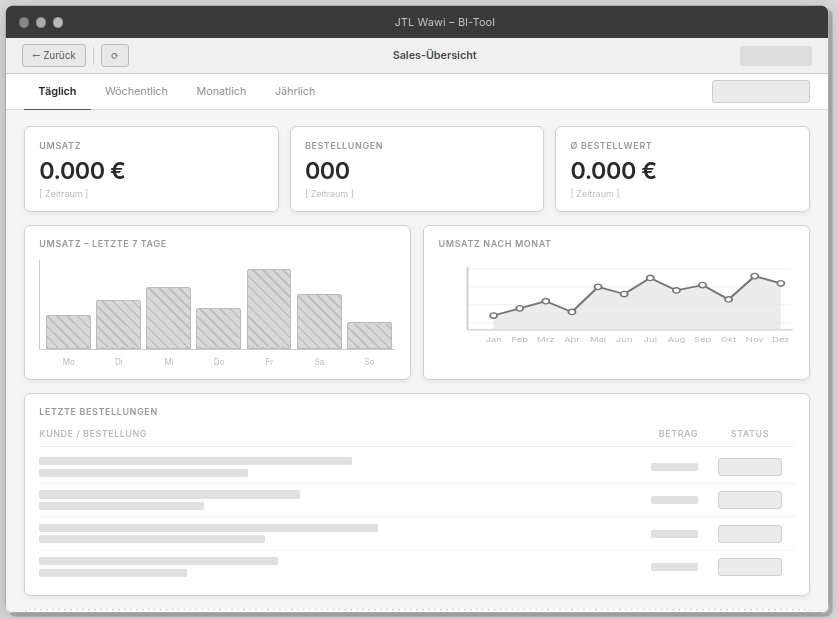
\includegraphics[width=0.85\textwidth]{image4}
  \caption{Mockup der Dashboard-Hauptansicht}
  \label{fig:mockup}
\end{figure}

\section{Pflichtenheft (Auszug)}
\label{anhang:pflichtenheft}

\textit{[Pflichtenheft-Auszug hier einfügen]}

\section{Iterationsplan}
\label{anhang:iterationsplan}

\begin{tabularx}{\textwidth}{l X r r r}
  \toprule
  \textbf{Iter.} & \textbf{Tätigkeit} & \textbf{Soll\,(h)} & \textbf{Ist\,(h)} & \textbf{Diff.} \\
  \midrule
  \multicolumn{5}{l}{\textit{Vorbereitung / Entwurfsphase}} \\
  \midrule
  1 & Einrichtung Monorepo-Struktur, TypeScript- und Vite-Konfiguration & 4 & [??????] & [??????] \\
  2 & Registrierung der App im JTL Developer Portal, API-Einrichtung & 3 & [??????] & [??????] \\
  \midrule
  \multicolumn{5}{l}{\textit{Implementierungsphase}} \\
  \midrule
  3 & Implementierung OAuth2-Authentifizierung (Backend, \texttt{getJwt}) & 5 & [??????] & [??????] \\
  4 & Implementierung Session-Token-Verifikation mit \gls{jwks} & 5 & [??????] & [??????] \\
  5 & Implementierung GraphQL-Proxy-Route (\texttt{/graphql}) & 4 & [??????] & [??????] \\
  6 & Implementierung generischer REST-Proxy (\texttt{/erp-info}) & 3 & [??????] & [??????] \\
  7 & Implementierung React-App-Routing und AppBridge-Integration & 5 & [??????] & [??????] \\
  8 & Implementierung Setup-Seite mit Token-Flow & 4 & [??????] & [??????] \\
  9 & Implementierung ERP-Dashboard: GraphQL-Datenabruf, KPI-Karten, Chart & 8 & [??????] & [??????] \\
  10 & Implementierung Pane-Widget mit Event-Subscription & 4 & [??????] & [??????] \\
  11 & Integration JTL Platform UI Komponenten, Styling & 5 & [??????] & [??????] \\
  12 & Funktionstests, Code Review, Fehlerbehebung & 8 & [??????] & [??????] \\
  \midrule
  \multicolumn{5}{l}{\textit{Dokumentation und Abschluss}} \\
  \midrule
  13 & Entwicklerdokumentation (JSDoc, Typisierungen) & 5 & [??????] & [??????] \\
  14 & Vorstellung, Abnahme, Abschluss & 2 & [??????] & [??????] \\
  \midrule
  & \textbf{Gesamt} & \textbf{65} & \textbf{[??????]} & \\
  \bottomrule
\end{tabularx}

\noindent\textit{Zuordnung zu den Projektphasen: Iter.~1–2 (7\,h) gehören zur Entwurfsphase
(Gesamtbudget Entwurf: 12\,h); Iter.~3–12 (51\,h) zur Implementierungsphase;
Iter.~13 (5\,h) zur Dokumentationsphase; Iter.~14 (2\,h) zur Abschlussphase.
Die Analysephase (10\,h) ist im Iterationsplan nicht enthalten, da sie keine
iterativen Entwicklungsschritte umfasst. Die Ist-Zeiten und Differenzen sind
nach Projektabschluss einzutragen.}

\section{Quellcode-Auszüge}
\label{anhang:quellcode}

Nachfolgend sind die zentralen Quellcode-Auszüge des Projekts dokumentiert.

\subsection{Backend: OAuth2-Token-Anfrage}

\begin{lstlisting}[language=JavaScript, caption={OAuth2-Token-Anfrage mit Basic Auth (index.ts)}, label=lst:oauth]
export async function getJwt(): Promise<string> {
  const authString = Buffer.from(
    `${process.env.CLIENT_ID}:${process.env.CLIENT_SECRET}`
  ).toString('base64');

  const response = await fetch(
    'https://auth.jtl-cloud.com/oauth2/token',
    {
      method: 'POST',
      headers: {
        'Content-Type': 'application/x-www-form-urlencoded',
        'Authorization': `Basic ${authString}`,
      },
      body: new URLSearchParams({ grant_type: 'client_credentials' }),
    }
  );
  const data = await response.json();
  if (response.ok) return data.access_token;
  throw new Error(`JWT-Fehler: ${data.error}`);
}
\end{lstlisting}

\subsection{Backend: Session-Token-Verifikation}

\begin{lstlisting}[language=JavaScript, caption={Session-Token-Verifikation mit JWKS (index.ts)}, label=lst:tokenmanager]
import { importJWK, jwtVerify } from 'jose';

const JWKS_URL =
  'https://api.jtl-cloud.com/account/.well-known/jwks.json';

async function verifySessionToken(
  sessionToken: string
): Promise<SessionTokenPayload> {
  const jwt = await getJwt();
  const response = await fetch(JWKS_URL, {
    headers: { Authorization: `Bearer ${jwt}` },
  });
  const jwks = await response.json();
  const publicKey = await importJWK(jwks.keys[0], 'EdDSA');
  const { payload } = await jwtVerify(sessionToken, publicKey);
  return payload as SessionTokenPayload;
}
\end{lstlisting}

\subsection{Backend: ERP-API-Proxy-Route}

\begin{lstlisting}[language=JavaScript, caption={Generischer REST-Proxy-Endpunkt (index.ts)}, label=lst:apiservice]
app.all('/erp-info/:tenantId/:endpoint',
  async (req: Request, res: Response) => {
    const { tenantId, endpoint } = req.params;
    const jwt = await getJwt();
    const options: RequestInit = {
      method: req.method,
      headers: {
        'X-Tenant-ID': tenantId,
        'Authorization': `Bearer ${jwt}`,
        'Content-Type': 'application/json',
      },
    };
    if (['POST', 'PUT', 'PATCH'].includes(req.method))
      options.body = JSON.stringify(req.body);
    const erpResponse = await fetch(
      `https://api.jtl-cloud.com/erp/${endpoint}`, options
    );
    if (erpResponse.ok) res.json(await erpResponse.json());
    else res.status(erpResponse.status).send(await erpResponse.text());
  }
);
\end{lstlisting}

\subsection{Backend: Tenant-Mapping}

\begin{lstlisting}[language=JavaScript, caption={Tenant-Mapping Endpunkt (index.ts)}]
const myMappingDatabase = new Map<string, string>();

app.post('/connect-tenant', async (req, res) => {
  const { sessionToken } = req.body;
  const payload = await verifySessionToken(sessionToken);
  const tenantId = new Date().getTime().toString();
  myMappingDatabase.set(tenantId, payload.tenantId);
  res.send(`Tenant ${tenantId} verbunden`);
});
\end{lstlisting}

\subsection{Frontend: App-Routing}

\begin{lstlisting}[language=JavaScript, caption={App-Komponente mit URL-basiertem Routing (App.tsx)}, label=lst:dashboard]
const App: React.FC<{ appBridge: AppBridge }> = ({ appBridge }) => {
  const mode = location.pathname.substring(1) as AppMode;
  switch (mode) {
    case 'setup': return <SetupPage appBridge={appBridge} />;
    case 'erp':   return <ErpPage   appBridge={appBridge} />;
    case 'pane':  return <PanePage  appBridge={appBridge} />;
    default:      return <div>Unknown mode</div>;
  }
};
\end{lstlisting}

\subsection{Frontend: Setup-Seite}

\begin{lstlisting}[language=JavaScript, caption={Setup-Seite mit AppBridge-Token-Flow (SetupPage.tsx)}, label=lst:setuppage]
const SetupPage: React.FC<ISetupPageProps> = ({ appBridge }) => {
  const [isLoading, setIsLoading] = useState(false);

  const handleSetupCompleted = useCallback(async () => {
    setIsLoading(true);
    const sessionToken = await appBridge.method.call('getSessionToken');
    const response = await fetch('/connect-tenant', {
      method: 'POST',
      headers: { 'Content-Type': 'application/json' },
      body: JSON.stringify({ sessionToken }),
    });
    if (response.ok)
      await appBridge.method.call('setupCompleted');
    setIsLoading(false);
  }, [appBridge]);

  return (
    <div>
      <h1>Setup</h1>
      <Button onClick={handleSetupCompleted} label="App verbinden" />
    </div>
  );
};
\end{lstlisting}

\subsection{Frontend: Pane-Widget}

\begin{lstlisting}[language=JavaScript, caption={Pane-Widget mit Event-Subscription (PanePage.tsx)}, label=lst:panepage]
const PanePage: React.FC<IPanePageProps> = ({ appBridge }) => {
  const [customer, setCustomer] = useState<string>();

  useEffect(() => {
    const unsubscribe = appBridge.event.subscribe(
      'CustomerChanged',
      (data: { customerId: string }) => {
        setCustomer(data.customerId);
        return Promise.resolve();
      }
    );
    return () => unsubscribe();
  }, [appBridge]);

  return (
    <Stack spacing="4" direction="column">
      <Text align="center" type="h2">Pane App</Text>
      <Input disabled value={customer} />
      <Button
        variant="outline"
        onClick={() => appBridge.method.call('getCurrentCustomerId')
          .then(id => setCustomer(id as string))}
        label="Aktuellen Kunden abrufen"
      />
    </Stack>
  );
};
\end{lstlisting}

\subsection{Frontend: ERP-Dashboard-Komponente}

\begin{lstlisting}[language=JavaScript,
  caption={ERP-Dashboard: Datenabruf und Darstellung (ErpPage.tsx, Auszug)},
  label=lst:erppage]
const ErpPage: React.FC<IErpPageProps> = ({ appBridge }) => {
  const [data, setData] = useState<DashboardData | null>(null);

  const load = useCallback(async () => {
    const token = await appBridge.method.call<string>('getSessionToken');
    const result = await fetchDashboard(token, computeDateRange('daily'));
    setData(result);
  }, [appBridge]);

  useEffect(() => { load(); }, [load]);

  return (
    <div className="flex flex-col gap-4 p-4 bg-gray-50">
      <div className="flex gap-3">
        <KpiCard label="Umsatz" value={formatEur(data.kpis.totalRevenue)} />
        <KpiCard label="Bestellungen" value={String(data.kpis.totalOrders)} />
      </div>
      <BarChart data={data.revenuePoints.slice(-7)}>
        <Bar dataKey="revenue" fill="#1a56db" />
      </BarChart>
      {data.recentOrders.slice(0, 8).map(order => (
        <div key={order.salesOrderNumber}>
          <p>{order.companyName}</p>
          <p>{formatEur(order.totalGrossAmount)}</p>
          <StatusBadge status={order.status} />
        </div>
      ))}
      <p>Avg. Bestellwert: {formatEur(data.kpis.avgOrderValue)}</p>
    </div>
  );
};
\end{lstlisting}

\subsection{Frontend: React-Einstiegspunkt}

\begin{lstlisting}[language=JavaScript, caption={main.tsx mit AppBridge-Initialisierung}]
import { createAppBridge } from '@jtl-software/cloud-apps-core';
import { StrictMode } from 'react';
import { createRoot } from 'react-dom/client';
import App from './App.tsx';

const appBridge = createAppBridge();

createRoot(document.getElementById('root')!).render(
  <StrictMode>
    <App appBridge={appBridge} />
  </StrictMode>
);
\end{lstlisting}

\section{Screenshot der Anwendung}
\label{anhang:screenshot_app}

\begin{figure}[H]
  \centering
  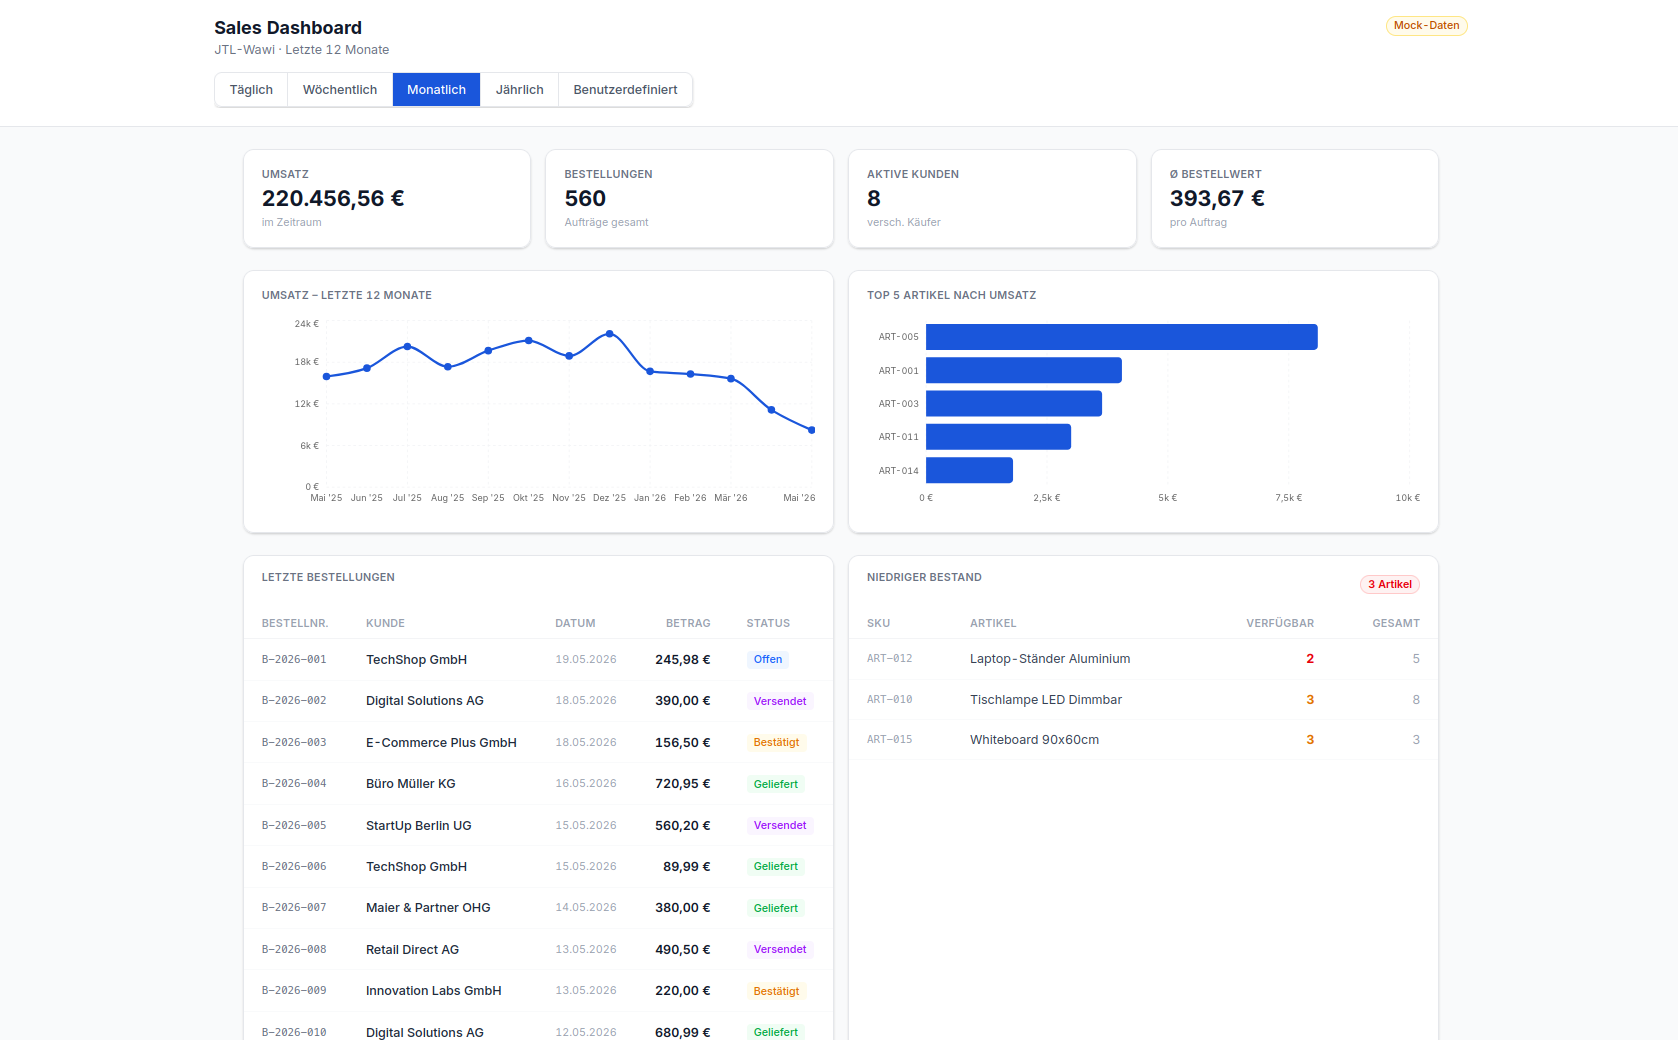
\includegraphics[width=0.95\textwidth]{image}
  \caption{Screenshot des fertigen ERP-Dashboards}
  \label{fig:screenshot_app}
\end{figure}

\section{Entwicklerdokumentation}
\label{anhang:entwicklerdoku}

Die Entwicklerdokumentation wurde mithilfe von TypeScript-Typisierungen und
JSDoc-Kommentaren erstellt. Nachfolgend die dokumentierten Backend-Funktionen:

\begin{lstlisting}[language=JavaScript, caption={TypeScript-Dokumentation (Backend)}]
/**
 * Verifiziert ein Session-Token und extrahiert die Payload.
 * Nutzt das JWKS vom JTL-Auth-Server zur EdDSA-Verifikation.
 *
 * @param sessionToken - Das zu verifizierende JWT
 * @returns Promise mit userId und tenantId
 * @throws Error bei ungueltigem Token
 */
async function verifySessionToken(
  sessionToken: string
): Promise<SessionTokenPayload> {
  // Implementierung...
}

/**
 * Ruft ein OAuth2 Access-Token vom JTL-Auth-Server ab.
 * Verwendet den client_credentials Grant-Type.
 *
 * @returns Promise mit dem Access-Token-String
 * @throws Error bei fehlenden Credentials oder API-Fehler
 */
export async function getJwt(): Promise<string> {
  // Implementierung...
}
\end{lstlisting}

\section{Eigenständigkeitserklärung}

\vspace{0.5cm}
Ich versichere hiermit, dass ich die vorliegende Projektarbeit selbstständig und
ohne unzulässige fremde Hilfe angefertigt habe. Alle Stellen, die ich wörtlich
oder sinngemäß aus veröffentlichten oder nicht veröffentlichten Quellen entnommen
habe, sind als solche kenntlich gemacht.

Tätigkeiten, die nicht von mir selbst durchgeführt wurden, sind in der Dokumentation
ausdrücklich als Fremdleistung gekennzeichnet (insbesondere Code Review und
Abnahme durch Mitarbeitende der \gls{ris}).

Die Dokumentation wurde gemäß den Vorgaben der \gls{ihk} Regensburg erstellt und
enthält keine unternehmensinternen Informationen, die nicht zur Veröffentlichung
freigegeben sind.

\vspace{3cm}
\begin{tabular}{lll}
  \rule{5cm}{0.4pt} & \quad & \rule{7cm}{0.4pt} \\
  Ort, Datum        &       & Unterschrift \AutorName \\
\end{tabular}

\end{document}